% Copyright (c) 2014,2016 Casper Ti. Vector
% Public domain.

\chapter{对RH代码的修改与讨论}
\section{对RH代码的修改}
在附录的这一章节,我将简单介绍我对RH代码的一些修改。相关修改的方法和文件已经上传到GitHub上,有需要的读者可以从下面的链接访问这些内容。
\subsection{嵌入STARK-B数据库结果}
对于Stark致宽的修改全部集中在RH主文件夹的\texttt{broad.c},具体其实非常傻瓜就是找到你要修改的能级,然后把它的Stark致宽计算公式修改成你想要的。这里提供了我修改了Mg \textsc{ii} h,k还有三重线Stark致宽的\texttt{broad.c}文件:

\url{https://github.com/nightmarein13/RH-SB}
\subsection{提供辐射流量输出}
RH1D代码中原本是存在辐射流量输出的(或者说一开始就设计成先求解辐射流量,如果有需求再去求解辐射强度),但是RH1.5D不知道为什么莫名其妙把它给删了,可能是Tiago觉得算太阳没必要看辐射流量?但是对于恒星耀斑的计算辐射流量还是相当重要的,因此需要花一些功夫把它加回来。具体的流程写在这个里面了:

\url{https://github.com/nightmarein13/my_toys/blob/master/add_flux.md}

修改后会在输出的HDF5文件中多生成一个名为\texttt{flux}的\texttt{dataset}。如果你使用Tiago提供的\texttt{helita}库中的\texttt{rh15d.Rh15dout()}类来读取输出,那么会自动在\texttt{ray}下生成一个名为\texttt{flux}的\texttt{xarray.DataArray}。
\subsection{用于修改大气的可视化Ipython Notebook}\label{sec:a.1.3}
大致是长图~\ref{fig:a.1.2}这个样子的,可以对温度、电子密度、一维速度和微湍动速度做一个简单(简陋)的调节。代码内容大量参考\texttt{helita}库中的\texttt{rh15d\_vis.InputAtmosphere()}类。下载地址:

\url{https://github.com/nightmarein13/my_toys/blob/master/rh15d_edit_atmos.py}

\begin{figure}
	\centering
	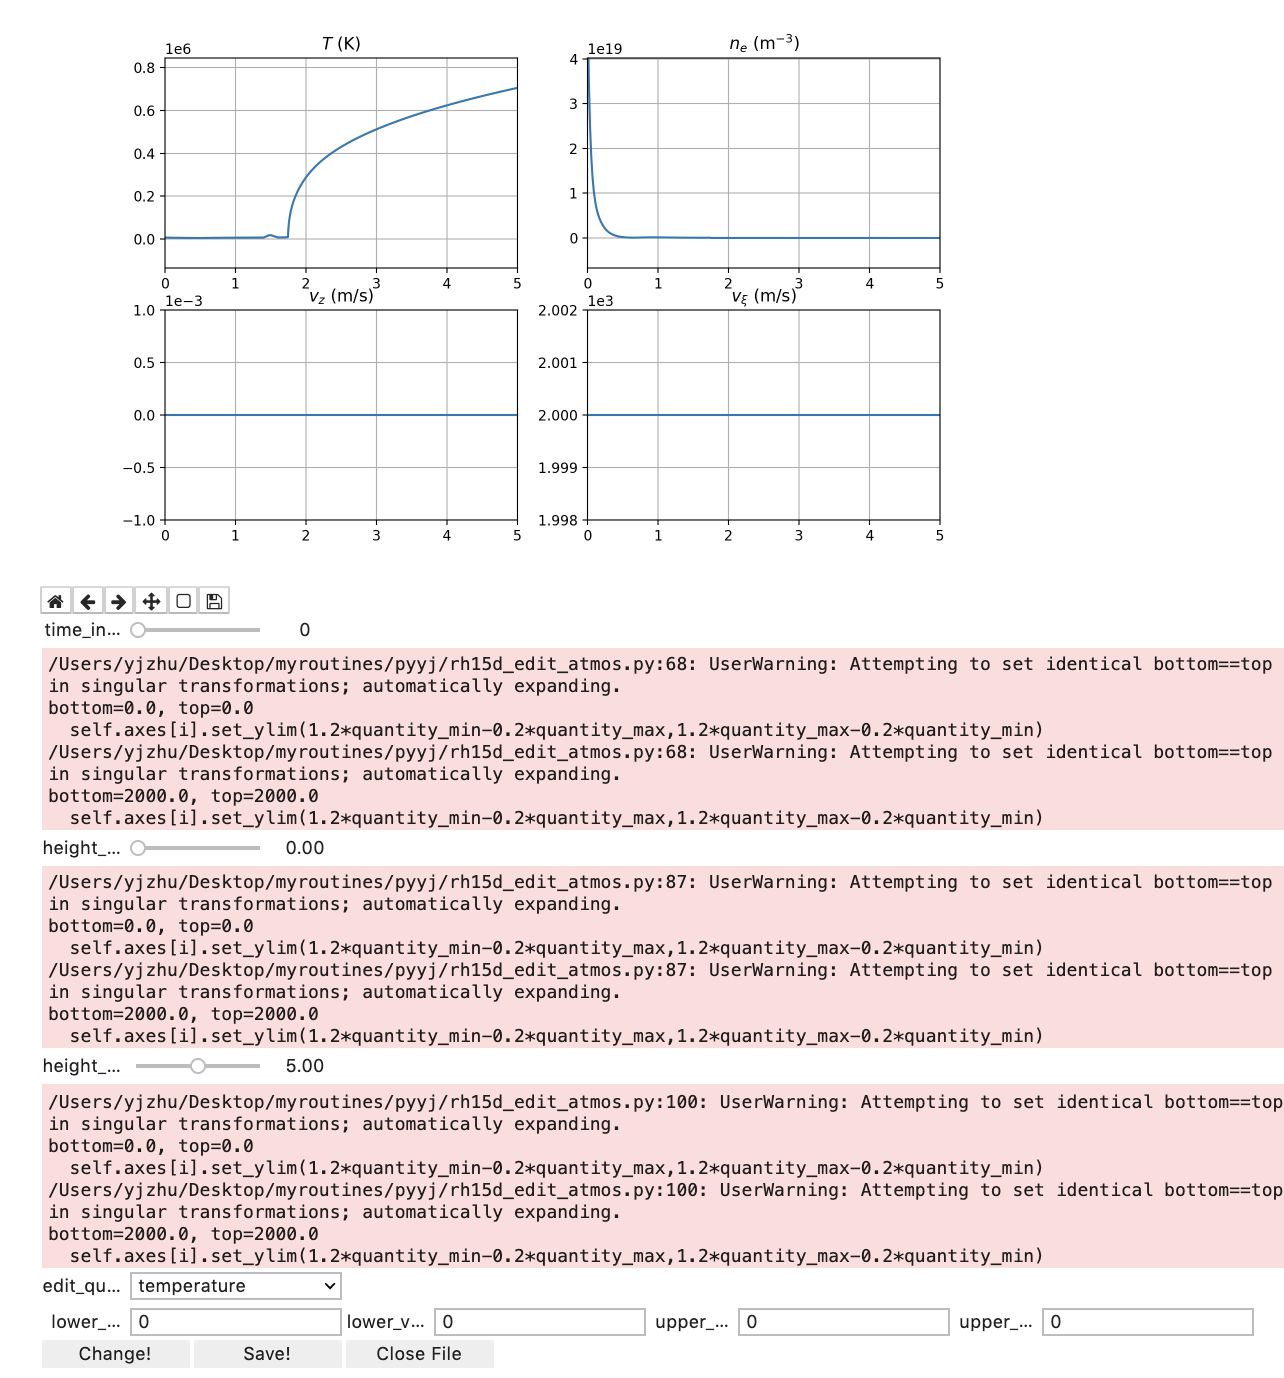
\includegraphics[width=\textwidth]{figs/naive}
	\caption{简陋的不能再简陋的可视化调节程序。。原谅我warning太多}
	\label{fig:a.1.2}
\end{figure}

\section{RH对Mg \textsc{ii}的Stark致宽的处理究竟有哪些问题?}\label{sec:a.2}
你要是问我到底该怎么算Stark致宽最好,那肯定从量子力学出发最好,但是毕竟像我这种不自量力的人是不会从微扰论出发算那么多矩阵元来求整个致宽问题的。因此我觉得有一些经典近似其实是很正常的。那么RH所做的经典碰撞近似究竟出了哪些问题呢?

根据\textcites{Mihalas2014}经典碰撞必须要满足三个条件才可能成立:

\textbf{碰撞持续时间和碰撞间隔的比较}

首先我们得定义一下碰撞持续时间,是碰撞过程中的总相移$\eta(\rho)$除以碰撞中最近时刻的频率移动,即\parencites{Mihalas2014}:
\begin{equation}
	\tau_{s}=\frac{\eta\left(\rho_{0}\right)}{\Delta \omega\left(\rho_{0}\right)}=\frac{\pi}{2} \cdot \frac{\rho_{0}}{v_{r e l}}
\end{equation}
其中等效瞄准距离$\rho_{0}=\left(\pi C_{4} / 2 v_{r e l}\right)^{1 / 3}$。

在碰撞近似之中,我们每次只考虑一个碰撞粒子对辐射粒子的作用,因此你的碰撞持续时间应该远小于碰撞间隔,即$\tau_s \ll \tau $。简单的来说就是你的等效瞄准距离$\rho_0$要比平均每个辐射粒子之间的间距$r_0$要小很多。对于Mg \textsc{ii}线心形成高度来说,$n_e \sim 10^{14}\ \mathrm{cm^{-3}}$,因此平均距离$r_0 \sim 10^{-5}\ \mathrm{cm}$。当我们取$T\sim 2\times 10^4$ K时,$\rho\sim 10^{-7}\ \mathrm{cm^{-3}}$。可见这条还是满足的,不然的话在经典框架内就只能去用统计理论算Holtzmark分布了。

\textbf{碰撞过程中的辐射}

碰撞近似忽略了碰撞过程中粒子发出的辐射,而这些辐射由于是在能级被扰动的情况下发出的,因此更有可能在线翼上,因此在远线翼上用碰撞近似本来就是不太好的,应该使用统计理论。一个典型的计算两个理论使用范围的分界频率是\parencites{Mihalas2014}:
\begin{equation}
	\Delta \omega_{c}=\frac{v_{r e l}^{4 / 3}}{(\pi / 2)^{4} C_{4}^{1 / 3}}
\end{equation}
对于电子产生的Stark致宽来说$\Delta \omega_{c}$远大于整个谱线轮廓,而对于离子来说如过取$C_4 \sim 10^{-14}-10^{-16}\ \mathrm{cm^4\cdot s^{-1}}$,$\Delta \omega_{c}\sim 0.5 -2.0$ \mbox{\AA}。因此其实Mg \textsc{ii}受离子的Stark致宽应该用统计理论来算,不过鉴于它相对于电子其实贡献并不多,可以暂时忽略。

\textbf{绝热近似}

由于碰撞理论是个纯经典的理论,我们希望整个碰撞持续时间所对应的频率$\omega_s = 1/\tau_s$要远远小于量子跃迁的频率,即\parencites{Mihalas2014}:
\begin{equation}
	\Delta \omega_{s} \ll \frac{E_{j}-E_{i}}{\hbar}
\end{equation}
对于Mg \textsc{ii}由自由电子引起的Stark效应,$\omega_s\sim 10^{15}\ \mathrm{rad\cdot s^{-1}}$。而Mg \textsc{ii} h和k线跃迁频率$\omega_{ij}\sim 6.7\times 10^{15}\ \mathrm{rad\cdot s^{-1}}$。两者在同一个量级上,所以我们认为绝热近似这个条件在此时是不满足的,还是需要引入STARK-B中考虑了部分量子力学效应的半经典理论来计算。



% vim:ts=4:sw=4
